\ChapterImageStar[cap:pmv]{Producto Mínimo Viable}{./images/fondo.png}\label{cap:pmv}
\mbox{}\\
\section{Estructura del proyecto}
\noindent
La figura~\ref{fig:estructura-proyecto} detalla la estructura del proyecto, el directorio functional-tests contiene los scripts y manifiestos utilizados para la validación técnica de la solución propuesta, el código fuente de esta validación puede encontrarse en la sección~\ref{sec:functional-tests}. 
\begin{figure}[H]
    \centering
    \begin{minipage}{0.48\textwidth}
        \centering
        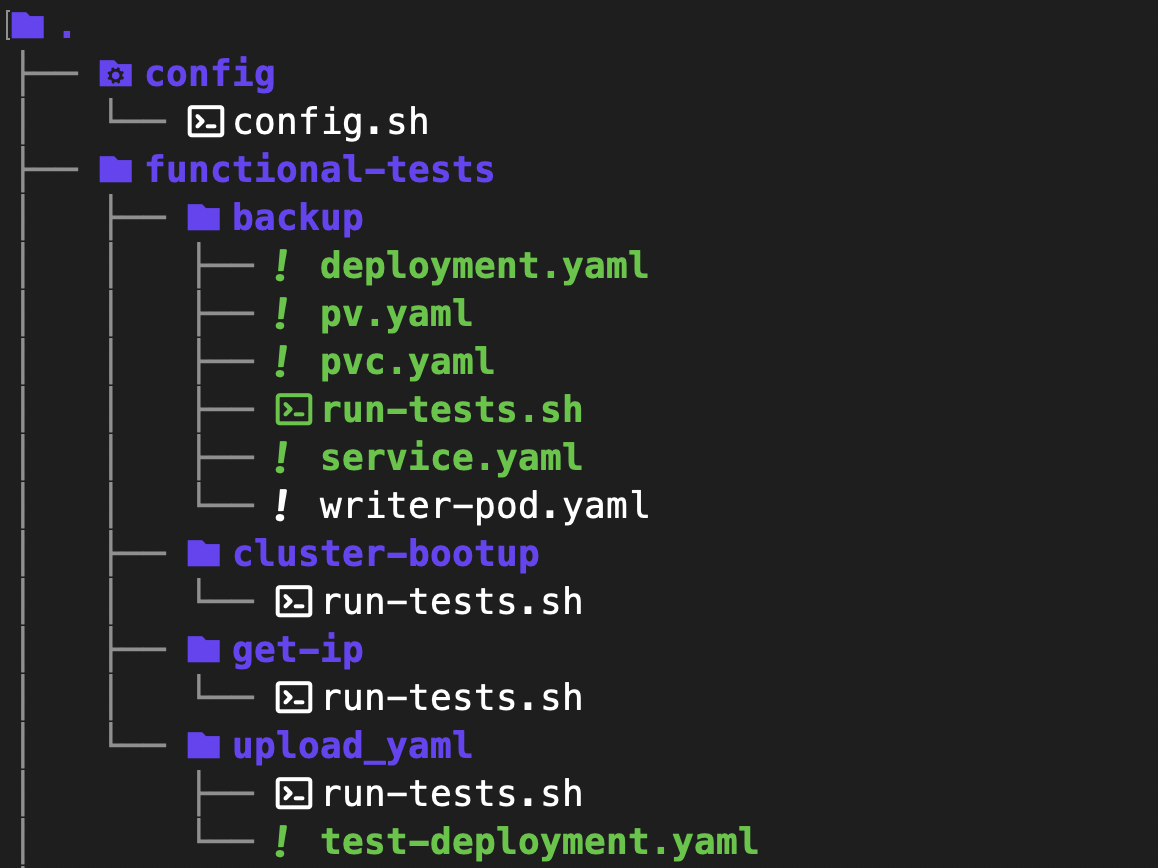
\includegraphics[scale=0.35]{tablas-images/cp6/src/tree-1.png}
        \subcaption{Parte 1}\label{fig:estructura-proyecto-1}
    \end{minipage}
    \hfill
    \begin{minipage}{0.48\textwidth}
        \centering
        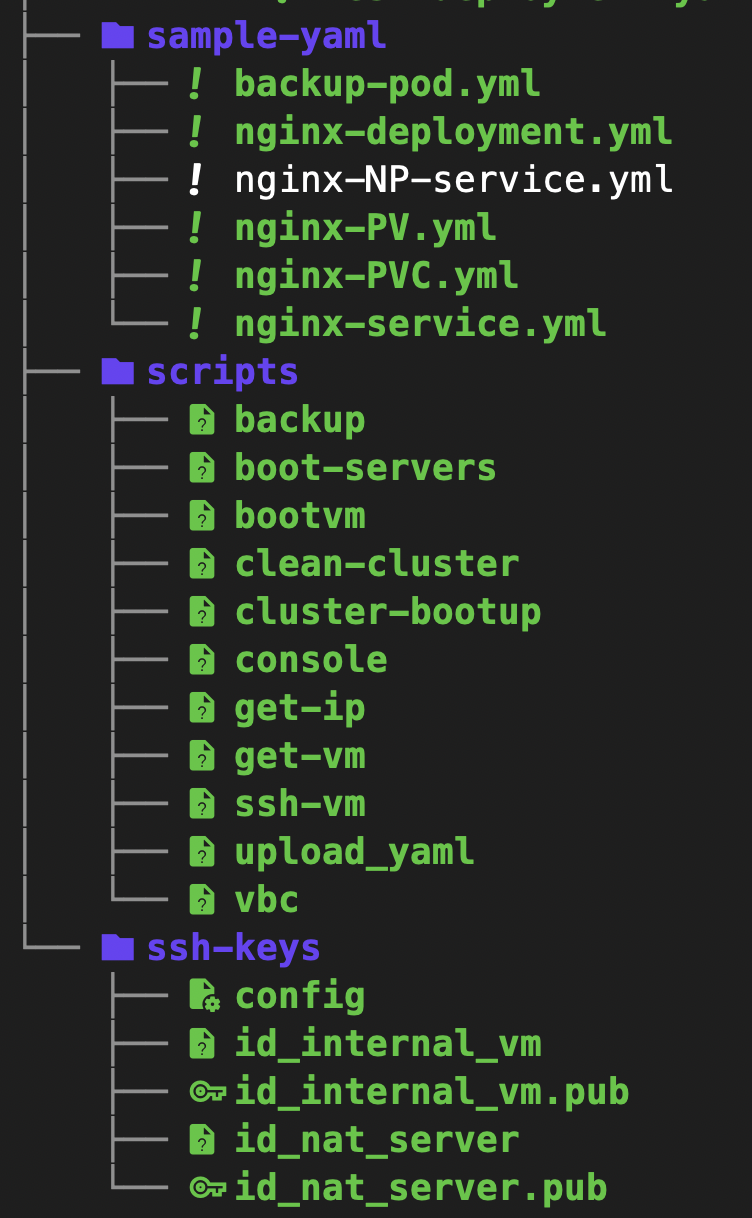
\includegraphics[scale=0.35]{tablas-images/cp6/src/tree-2.png}
        \subcaption{Parte 2}\label{fig:estructura-proyecto-2}
    \end{minipage}
    \caption{Estructura del proyecto}\label{fig:estructura-proyecto}
\end{figure}

\section{Código fuente}\label{sec:automatizacion-scripts}
\noindent
El código fuente del sistema, desarrollado en el lenguaje Bash, está disponible en el repositorio de GitHub \href{https://github.com/AariazP/TG-VBC.git}{\texttt{TG-VBC}} en la rama \texttt{scripted-solution}. Este repositorio contiene scripts para la automatización de tareas en la infraestructura de virtualización basada en contenedores, incluyendo la configuración de nodos, despliegue de \VM\ y configuración de Kubernetes. 

\subsection{Config}
\noindent
Este paquete contiene scripts de configuración y utilidades para la gestión de máquinas virtuales en un entorno XCP-ng.
%=========================CONFIG=========================
\subsubsection{Config.sh}
\noindent
El siguiente script en \textit{bash} tiene como finalidad modificar la tabla de enrutamiento del sistema mediante la adición de una ruta estática. 
De esta manera, se define un camino específico para que los paquetes dirigidos a la red \texttt{192.168.100.0/24} sean encaminados a través de la 
puerta de enlace \texttt{172.30.29.2}, utilizando la interfaz de red \texttt{xenbr0}. 
Este tipo de configuración es común en entornos de virtualización como Xen o XCP-ng, donde los bridges de red permiten interconectar  máquinas virtuales con la red física.

\begin{minted}[frame=lines,
    fontsize=\scriptsize,
    breaklines]{bash}
#!/bin/bash

# Agrega una ruta estática a la tabla de enrutamiento del sistema.
# En este caso, se está indicando que para llegar a la red 192.168.100.0/24 
# (es decir, todas las IP desde 192.168.100.1 hasta 192.168.100.254 con máscara /24),
# el tráfico debe enviarse a través de la puerta de enlace 172.30.29.2,
# utilizando la interfaz de red xenbr0 (un bridge, normalmente en entornos con Xen o XCP-ng).
sudo ip route add 192.168.100.0/24 via 172.30.29.2 dev xenbr0
\end{minted}

%=========================SAMPLE-YAML=========================

\subsection{sample-yaml}
\noindent
Los archivos en formato \texttt{YAML} presentados en esta sección son ejemplos utilizados en diferentes contextos del PMV, incluyendo la configuración de pods, despliegues, servicios y volúmenes persistentes en Kubernetes. Estos manifiestos sirven como referencia para la creación y gestión de recursos dentro del clúster, facilitando la implementación de aplicaciones y servicios de manera eficiente y estructurada.
Se pueden encontrar en el apéndice~\ref{apendice:yaml-pmv}.


%=========================SCRIPTS=========================
\subsection{Scripts}

\subsection{backup.sh}
\noindent
\begin{minted}[frame=lines,
    fontsize=\scriptsize,
    breaklines]{bash}
#!/bin/bash

# ensures file cleanup after cancellation

trap "rm -f exporter_file.yaml" SIGINT

MODE="pvc"
TARGET=""
POD=""
FOLDER=""
while getopts "p:f:" opt; do
  case "$opt" in
    p) MODE="pod"; POD="$OPTARG" ;;     # backup from pod:path
    f) MODE="folder"; FOLDER="$OPTARG" ;; # backup from host path
  esac
done
shift $((OPTIND-1))

NODE="$( get-vm -a -n 1 master )"

PVC="$1"
DATE=$( date +%Y-%m-%d-%H-%M-%S-%s )

if [[ "$MODE" == "pvc" ]]; then
  # --- current PVC backup flow ---
  cat <<EOF > exporter_file.yaml
apiVersion: v1
kind: Pod
metadata:
  name: exporter
spec:
  containers:
  - name: exporter
    image: alpine
    command: ["sleep", "3600"]
    volumeMounts:
    - mountPath: /data
      name: export-pvc
  volumes:
  - name: export-pvc
    persistentVolumeClaim:
      claimName: ${PVC}
EOF

  upload_yaml ${NODE} exporter_file.yaml

  while [[ $(ssh-vm -r ${NODE} -c "kubectl get pod/exporter -o jsonpath='{.status.phase}'") != "Running" ]]; do
    sleep 1
  done
  FILENAME="/tmp/backup-${DATE}-pvc.tar"
  ssh-vm -r ${NODE} -c "kubectl cp exporter:/data ./backup-${DATE}"
  ssh-vm -r ${NODE} -c "kubectl delete pod/exporter"
  ssh-vm -r ${NODE} -c "tar -cvf ${FILENAME} ./backup-${DATE}"

elif [[ "$MODE" == "pod" ]]; then
  FILENAME="/tmp/backup-${DATE}-pod.tar"
  # --- backup arbitrary path from pod ---
  ssh-vm -r ${NODE} -c "kubectl cp ${POD} ./backup-${DATE}"
  ssh-vm -r ${NODE} -c "tar -cvf ${FILENAME} ./backup-${DATE}"

elif [[ "$MODE" == "folder" ]]; then
  FILENAME="/tmp/backup-${DATE}-node.tar"
  # --- backup arbitrary folder from node ---
  NODE=$( echo $FOLDER | cut -d":" -f1 )
  FOLDER=$( echo $FOLDER | cut -d":" -f2 ) 
  echo "++++++ $NODE ++++ $FOLDER +++"
  ssh-vm -r ${NODE} -c "tar -cvf ${FILENAME} ${FOLDER}"
fi

exec 2>/dev/null
scp -i ~/.ssh/id_internal_vm root@$(get-ip ${NODE}):"${FILENAME}" ./

rm -f exporter_file.yaml
\end{minted}

\subsection{boot-servers.sh}
\noindent
El script \texttt{boot-servers.sh} tiene como finalidad automatizar la creación e inicialización de máquinas virtuales, específicamente servidores que cumplen el rol de red \texttt{NAT}. El funcionamiento contempla dos escenarios: la creación de un servidor NAT principal (\textit{Master}) y, de manera opcional, un servidor de respaldo (\textit{Backup}) a partir de una plantilla predefinida denominada \texttt{nat-server}. Una vez creadas las máquinas virtuales, el script procede a encenderlas utilizando las utilidades nativas de XCP-ng,  permitiendo que la infraestructura de red NAT esté disponible.

\begin{minted}[frame=lines,
    fontsize=\scriptsize,
    breaklines]{bash}
#!/bin/bash

# ---------------------------------------------------------------
# Script: boot-servers.sh
# Descripción:
#   Este script crea e inicia las máquinas virtuales principales 
#   de red NAT en XCP-ng. Puede crear un servidor NAT principal 
#   (Master) y, opcionalmente, un servidor de respaldo (Backup) 
#   usando plantillas predefinidas.
# ---------------------------------------------------------------

# Variable que indica si se debe crear el servidor de backup
BACKUP=0

# Procesar opciones:
#   -b  → crea el servidor NAT de backup adicional
while getopts "b" opt; do
  case $opt in
    b) BACKUP=1 ;;  # Activar creación del backup
    *) echo "Usage: $0 [-w NUM_WORKERS] [-m NUM_MASTERS] [-b NAT server backup?]" >&2
       exit 1 ;;
  esac
done

# Crear el servidor NAT principal (Master) a partir de la plantilla "nat-server"
MASTER_UUID=$(xe vm-install template="nat-server" new-name-label="NAT-Master")

# Si se indicó la opción -b, crear también el servidor de backup
[[ $BACKUP > 0 ]] && BACKUP_UUID=$(xe vm-install \
     template="nat-server" new-name-label="NAT-Backup")

# Iniciar la VM principal (Master)
xe vm-start uuid=$MASTER_UUID

# Esperar 2 segundos para dar tiempo a que arranque la Master
sleep 2

# Si se creó la VM de backup, iniciarla también
[[ $BACKUP > 0 ]] && xe vm-start uuid=$BACKUP_UUID
\end{minted}

\subsection{bootvm.sh}
\noindent
El script \texttt{bootvm.sh} permite automatizar la creación e inicio de una \VM\. Su funcionamiento parte de una plantilla predefinida, identificada por un \texttt{UUID}, desde la cual se instancia una nueva máquina virtual. El usuario debe proporcionar un nombre como argumento de entrada, el cual se asigna directamente a la \VM\ creada. Finalmente, el script arranca la máquina virtual recién generada de forma automática. 

\begin{minted}[frame=lines,
    fontsize=\scriptsize,
    breaklines]{bash}
#!/bin/bash

# ---------------------------------------------------------------
# Script: bootvm.sh
# Descripción:
#   Este script crea e inicia una máquina virtual (VM) en XCP-ng 
#   a partir de una plantilla predefinida, usando el nombre que 
#   se le pase como argumento.
# ---------------------------------------------------------------

# Validar que se haya pasado al menos un argumento (nombre de la VM)
if [ $# -lt 1 ]
then
   echo "usage: bootvm <vm-name>"
   exit 0
fi

# Crear la VM a partir de una plantilla específica (UUID de la plantilla)
# y asignarle un nombre nuevo igual al argumento pasado
VM_UUID=$(xe vm-install template=0c838875-cb93-dfe3-8c36-a2f42183b434 \
           new-name-label="$1")

# Iniciar la VM recién creada usando su UUID
xe vm-start uuid=$VM_UUID
\end{minted}

\subsection{clean-cluster.sh}
\noindent
\begin{minted}[frame=lines,
    fontsize=\scriptsize,
    breaklines]{bash}
#!/bin/bash

# ---------------------------------------------------------------
# Script: clean-cluster.sh
# Descripción:
#   Este script elimina todas las máquinas virtuales (VMs) de un 
#   cluster en XCP-ng, excluyendo dominios del sistema. Puede 
#   ejecutarse de manera interactiva o automática usando la opción -y.
# ---------------------------------------------------------------

# Variable que indica si se debe asumir "sí" automáticamente
ASSUME_YES=false

# ---------------------------------------------------------------
# Procesar opción:
#   -y  → Asumir "sí" automáticamente para borrar las VMs
# ---------------------------------------------------------------
while getopts "y" opt; do
  case $opt in
    y)
      ASSUME_YES=true  # Activar borrado automático
      ;;
    *)
      echo "Usage: $0 [-y]"
      exit 1
      ;;
  esac
done

# Si no se asumió "sí", pedir confirmación al usuario
if [ "$ASSUME_YES" = false ]; then
  read -p "Are you really sure you want to clean cluster. (y/N): " resp
  [[ ! $resp =~ (y|Y|yes|Yes|YES) ]] && exit 0
fi

# Obtener lista de VMs a eliminar, excluyendo dominios del sistema
vms=$(xe vm-list | grep name-label | grep -v "domain" | grep -oP "(?<=: ).+")

# Iterar sobre cada VM encontrada
for vm in $vms; do
  # Obtener UUID de la VM
  UUID=$(xe vm-list name-label="$vm" --minimal | tr ',' ' ')
  
  # Apagar la VM de forma forzada en segundo plano
  xe vm-shutdown uuid=$UUID force=true &
  wait $!  # Esperar a que termine el apagado
  
  # Eliminar la VM del sistema
  xe vm-destroy uuid=$UUID
done
\end{minted}

\subsection{cluster-bootup.sh}
\noindent
\begin{minted}[frame=lines,
    fontsize=\scriptsize,
    breaklines]{bash}
#!/bin/bash

# ---------------------------------------------------------------
# Script: cluster-bootup.sh
# Descripción:
#   Este script crea e inicializa un cluster K3s en XCP-ng, 
#   desplegando servidores master, workers, y opcionalmente 
#   un load balancer y un servidor NAT de backup. Configura 
#   hostnames, IPs, HAProxy (si hay load balancer) y une 
#   todos los nodos al cluster.
# ---------------------------------------------------------------

# Valores por defecto
NUM_WORKERS=2
NUM_MASTERS=1
BACKUP=0
HAS_LB=0

# Procesar opciones:
# -w NUM_WORKERS  → Número de nodos worker
# -m NUM_MASTERS  → Número de nodos master
# -b              → Crear NAT server backup
while getopts "w:m:b" opt; do
  case $opt in
    w) NUM_WORKERS=$OPTARG ;;
    m) NUM_MASTERS=$OPTARG ;;
    b) BACKUP=1 ;;
    *) echo "Usage: $0 [-w NUM_WORKERS] [-m NUM_MASTERS] [-b NAT server backup?]" >&2
       exit 1 ;;
  esac
done

# Si hay más de un master, se necesitará un load balancer
[[ $NUM_MASTERS > 1 ]] && HAS_LB=1 

# Crear servidores NAT (Master y opcionalmente Backup)
[[ $BACKUP > 0 ]] &&  boot-servers -b ||  boot-servers 

# Esperar 3 segundos para que arranquen
sleep 3

# Definir nombres y cantidad de nodos a crear
NAMES=( master worker )
VALUES=( $NUM_MASTERS $NUM_WORKERS )

# Si hay load balancer, agregarlo al arreglo
if [[ $HAS_LB > 0 ]]; then
    NAMES=( load-balancer master worker )
    VALUES=( 1 $NUM_MASTERS $NUM_WORKERS )
fi

# Crear VMs según tipo y cantidad
for idx in $( seq 0 ${#NAMES[@]} | head -n -1 ); do
    name=${NAMES[$idx]}
    value=${VALUES[$idx]} 

    # Crear cada VM del tipo correspondiente
    for i in $( seq 1 $value ); do
        bootvm $name$i
    done

    sleep 2

    # Configurar hostname y /etc/hosts en cada VM
    for i in $( seq 1 $value ); do
        echo "=== setting up $name$i hostname ==="
        
        # Esperar a que la VM tenga IP
        while [ -z $VM_IP ]; do 
            VM_IP=$( get-ip $name$i )
            sleep 1
        done

        # Configurar hostname remoto
        ssh -i ~/.ssh/id_internal_vm root@$VM_IP \
            "hostnamectl set-hostname $name$i; hostname; \
             echo '127.0.0.1 $name$i' >> /etc/hosts"

        VM_IP=""
    done
done

# Obtener IP del master1
MASTER_IP=$( get-ip master1 )

# Obtener IP del load balancer si existe
[ $HAS_LB -gt 0 ] && LB_IP=$( get-ip load-balancer1 )

# Instalar K3s en master1
if [ $HAS_LB -gt 0 ]; then
    ssh -i ~/.ssh/id_internal_vm root@$MASTER_IP \
        "curl -sfL https://get.k3s.io | sh -s - server --cluster-init --tls-san ${LB_IP}"
else
    ssh -i ~/.ssh/id_internal_vm root@$MASTER_IP \
        "curl -sfL https://get.k3s.io | sh -"
fi

# Obtener token de cluster K3s para unir nodos
while [ -z $TOKEN ]; do
    TOKEN=$( ssh -i ~/.ssh/id_internal_vm root@$MASTER_IP \
             "sudo cat /var/lib/rancher/k3s/server/node-token" )
done

# Configurar HAProxy si hay load balancer
if [[ $HAS_LB > 0 ]]; then

    # Instalar HAProxy
    ssh -i ~/.ssh/id_internal_vm root@$LB_IP "apt install haproxy -y"

    # Configuración básica de HAProxy
    config="frontend k3s-api
        bind *:6443
        default_backend k3s-masters

    backend k3s-masters
        balance roundrobin
    "

    # Agregar cada master al backend de HAProxy
    for i in $( seq 1 $NUM_MASTERS ); do
        ip=$( get-ip master$i )
        config+="    server master${i} ${ip}:6443 check
"
    done

    # Mostrar configuración
    echo "_____________________"
    echo "$config"
    echo "_____________________"

    # Subir configuración al LB y reiniciar servicio
    ssh -i ~/.ssh/id_internal_vm root@$LB_IP \
        "cat > /etc/haproxy/haproxy.cfg" <<< "$config"
    ssh -i ~/.ssh/id_internal_vm root@$LB_IP "sudo systemctl restart haproxy"

fi

# Arreglos de nombres, cantidad y modos para unir nodos
NAMES=( master worker )
VALUES=( $NUM_MASTERS $NUM_WORKERS )
MODES=( "-s - server" "-" )

# Determinar IP a la que los nodos se unirán
JOIN_IP=${LB_IP}
[ $HAS_LB -eq 0 ] && JOIN_IP=$MASTER_IP

# Unir nodos al cluster K3s
for idx in {0..1}; do
    name=${NAMES[$idx]}
    value=${VALUES[$idx]}
    mode=${MODES[$idx]}

    for i in $( seq 1 $value ); do
        # Saltar master1 que ya está inicializado
        [[ ${name}${i} == "master1" ]] && continue

        echo "=== joining host $name$i to cluster ==="

        # Esperar a que la VM tenga IP
        while [ -z $VM_IP ]; do 
            VM_IP=$( get-ip $name$i )
            sleep 1
        done

        # Ejecutar script K3s para unir nodo al cluster
        ssh -i ~/.ssh/id_internal_vm root@$VM_IP \
            "curl -sfL https://get.k3s.io | K3S_URL=https://${JOIN_IP}:6443 K3S_TOKEN=${TOKEN} sh ${mode}"

        VM_IP=""
    done
done
\end{minted}

\subsection{console.sh}
\noindent
El siguiente script denominado \texttt{console.sh} implementa una interfaz en modo texto interactiva para la gestión de un cluster K3s. Utiliza la herramienta \texttt{whiptail} para mostrar menús, cuadros de entrada y listas de selección que permiten al usuario ejecutar operaciones comunes de forma sencilla. Entre sus funcionalidades se incluyen: subir archivos \texttt{YAML} a un nodo, limpiar el cluster eliminando las \VM, realizar respaldos en diferentes modalidades \texttt{(PVC, Pod o nodo)}, agregar nuevas \VM\ al cluster, establecer conexiones SSH con nodos específicos y desplegar un cluster completo definiendo el número de masters, workers y la opción de incluir un \NAT\ de respaldo. Este enfoque mejora la usabilidad al abstraer comandos complejos en un menú amigable que guía al usuario en cada paso.

\begin{minted}[frame=lines,
    fontsize=\scriptsize,
    breaklines]{bash}
#!/bin/bash

# ---------------------------------------------------------------
# Script: console.sh
# Descripción:
#   Proporciona una interfaz de menús en modo texto para la 
#   gestión de un cluster K3s en XCP-ng mediante la herramienta
#   'whiptail'. Permite ejecutar operaciones comunes como:
#   - Subir archivos YAML
#   - Limpiar el cluster
#   - Realizar backups
#   - Agregar nuevas VMs
#   - Conectar por SSH
#   - Inicializar el cluster
# ---------------------------------------------------------------

# Banner ASCII mostrado en el menú principal
read -r -d '' BANNER <<'EOF'
+-------------------------------------------------------+
|  _____ _____  _____ _____      __      ______   _____ |
| / ____|  __ \|_   _|  __ \     \ \    / /  _ \ / ____||
| |  __| |__) | | | | |  | |_____\ \  / /| |_) | |     ||
| | |_ |  _  /  | | | |  | |______\ \/ / |  _ <| |     ||
| |__| | | \ \ _| |_| |__| |       \  /  | |_) | |____ ||
| \_____|_|  \_\_____|_____/         \/   |____/ \_____||
|                                                       |
+-------------------------------------------------------+
EOF

# Configuración de colores para whiptail
export NEWT_COLORS='
root=white,blue'

# Bucle principal del menú
while true; do
    # Menú principal con whiptail
    choice=$(whiptail --title "Menú Principal" \
        --menu "$BANNER\nSeleccione una opción:" 30 62 10 \
        "1" "Subir archivo" \
        "2" "Limpiar cluster" \
        "3" "Backup" \
        "4" "Agregar VM al cluster" \
        "5" "SSH" \
        "6" "Inicializar cluster" \
        "7" "Salir" \
        3>&1 1>&2 2>&3)

    exitstatus=$?
    if [ $exitstatus -ne 0 ] || [ "$choice" == "7" ]; then
        echo "Saliendo..."
        break
    fi

    case $choice in
        # Subir archivo YAML a un nodo
        "1")
            node=$(whiptail --inputbox "Ingrese el nodo:" 10 60 3>&1 1>&2 2>&3)
            [ $? -ne 0 ] && continue
            file=$(whiptail --inputbox "Ingrese el archivo:" 10 60 3>&1 1>&2 2>&3)
            [ $? -ne 0 ] && continue
            echo "Ejecutando: upload_yaml $node $file"
            upload_yaml "$node" "$file"
            ;;
        # Limpiar cluster
        "2")
            echo "Ejecutando: clean-cluster"
            clean-cluster
            ;;
        # Opciones de backup
        "3")
            backup_choice=$(whiptail --title "Opciones de Backup" \
                --menu "Seleccione el tipo de backup:" 20 60 10 \
                "1" "Backup para PVC" \
                "2" "Backup para Pod" \
                "3" "Backup para Nodo" \
                3>&1 1>&2 2>&3)
            [ $? -ne 0 ] && continue

            case $backup_choice in
                "1")
                    pvc=$(whiptail --inputbox "Ingrese el PVC:" 10 60 3>&1 1>&2 2>&3)
                    [ $? -ne 0 ] && continue
                    echo "Ejecutando: backup-pvc $pvc"
                    backup "$pvc"
                    ;;
                "2")
                    pod_route=$(whiptail --inputbox "Ingrese el pod-route:" 10 60 3>&1 1>&2 2>&3)
                    [ $? -ne 0 ] && continue
                    echo "Ejecutando: backup-pod $pod_route"
                    backup -p "$pod_route"
                    ;;
                "3")
                    carpeta=$(whiptail --inputbox "Ingrese la carpeta:" 10 60 3>&1 1>&2 2>&3)
                    [ $? -ne 0 ] && continue
                    echo "Ejecutando: backup-nodo $carpeta"
                    backup -f "$carpeta"
                    ;;
            esac
            ;;
        # Agregar VM al cluster
        "4")
            vm_name=$(whiptail --inputbox "Ingrese el nombre de la VM:" 10 60 3>&1 1>&2 2>&3)
            [ $? -ne 0 ] && continue
            echo "Ejecutando: bootvm -j $vm_name"
            bootvm -j "$vm_name"
            ;;
        # Conexión SSH a una VM
        "5")
            vm_name=$(whiptail --inputbox "Ingrese el nombre de la VM:" 10 60 3>&1 1>&2 2>&3)
            [ $? -ne 0 ] && continue
            echo "Ejecutando: ssh-vm $vm_name"
            ssh-vm "$vm_name"
            ;;
        # Inicialización de un cluster completo
        "6")
            masters=$(whiptail --inputbox "Ingrese la cantidad de masters:" 10 60 3>&1 1>&2 2>&3)
            [ $? -ne 0 ] && continue
            workers=$(whiptail --inputbox "Ingrese la cantidad de workers:" 10 60 3>&1 1>&2 2>&3)
            [ $? -ne 0 ] && continue
            nat_backup=$(whiptail --title "Opciones adicionales" \
               --checklist "Seleccione si desea agregar NAT-Backup:" 15 60 5 \
               "1" "Agregar NAT-Backup" OFF \
               3>&1 1>&2 2>&3 )
            [ $? -ne 0 ] && continue

            [ $nat_backup -eq 1 ] && nat_backup="-b"

            echo "Ejecutando: cluster-bootup -m $masters -w $workers $nat_backup"
            cluster-bootup -m "$masters" -w "$workers" $nat_backup
            ;;
    esac
done
\end{minted}

\subsection{get-ip.sh}
\noindent
El script \texttt{get-ip.sh} tiene como finalidad obtener de manera automática la dirección IP de una \VM\, partiendo únicamente de su nombre. Para ello, se conecta al servidor \NAT\ a través de \texttt{SSH} utilizando una llave privada, consulta la tabla ARP mediante el comando \texttt{ip n}, y filtra las entradas que coinciden con las direcciones MAC asociadas a la \VM. De esta forma, el script permite resolver dinámicamente la IP de la \VM.

\begin{minted}[frame=lines,
    fontsize=\scriptsize,
    breaklines]{bash}
#!/bin/bash

# ---------------------------------------------------------------
# Script: get-ip.sh
# Descripción:
#   Este script obtiene la dirección IP de una máquina virtual 
#   (VM) en XCP-ng a partir de su nombre.
# ---------------------------------------------------------------

# Verificación de argumentos:
# Si no se pasa al menos un argumento (nombre de la VM), se muestra 
# el uso correcto del script y se termina.
if [ $# -lt 1 ]
then
   echo "usage: get-ip <vm-name>"
   exit 0
fi

# Caso especial: 
# Si el nombre de la VM es "NAT-Master", se devuelve una IP fija 
# sin necesidad de consultar nada en XCP-ng.
if [[ "$1" == "NAT-Master" ]]
then
   echo "172.30.29.2"
   exit 0
fi

# Obtiene el UUID de la VM en XCP-ng a partir del nombre de la VM.
VM_UUID=$( xe vm-list name-label="$1" --minimal )

# Obtiene las direcciones MAC de las interfaces de red (VIFs) 
# asociadas a la VM, separadas por coma.
VM_MAC=$( xe vif-list vm-uuid="$VM_UUID" params=MAC --minimal )

# Convierte la lista separada por comas en un arreglo de MACs. 
# Se asumen máximo dos interfaces de red.
MACS=( $( echo $VM_MAC | cut -d, -f1 ) $( echo $VM_MAC | cut -d, -f2 ) )

# Redirige los errores a /dev/null para evitar mostrar mensajes 
# de advertencia de ssh u otros.
exec 2> /dev/null

# Se conecta al servidor NAT (172.30.29.2) vía SSH usando una llave 
# privada, y ejecuta el comando `ip n` (vecinos en ARP/NDP).
# Luego filtra las líneas que contengan alguna de las MACs de la VM 
# y extrae la primera columna (la IP asociada).
VM_IP=$( ssh -i ~/.ssh/id_nat_server debian@172.30.29.2 \
        "ip n | fgrep -e ${MACS[0]} -e ${MACS[1]}" | cut -d" " -f1 )

# Muestra la IP obtenida sin salto de línea adicional al final.
echo -n $VM_IP
\end{minted}


\subsection{get-vm.sh}
\noindent
El siguiente script permite listar las máquinas virtuales disponibles y verificar cuáles se encuentran activas. Para ello, utiliza opciones de línea de comandos que permiten: (i) listar todas las máquinas virtuales, (ii) comprobar mediante \texttt{ping} la disponibilidad de una \VM\ específica, y (iii) limitar el número de resultados mostrados. El script hace uso de los comandos \texttt{xe} para obtener los nombres de las máquinas virtuales y combina utilidades como \texttt{ssh}, \texttt{timeout} y \texttt{grep} para gestionar el filtrado y la verificación de conectividad. 

\begin{minted}[frame=lines,
    fontsize=\scriptsize,
    breaklines]{bash}
#!/bin/bash

CHECK_ALL=0   # Variable que indica si se deben verificar todas las VMs
LIMIT=0       # Límite en el número de VMs a mostrar

# Procesa las opciones de línea de comandos
while getopts "ap:n:" opt; do
  case $opt in
    # -a: activa la verificación de todas las VMs
    a) CHECK_ALL=1 ;;
    # -p <vm_name>: comprueba mediante ping si la VM indicada responde
    p) ssh-vm NAT-Master -c "timeout 3 ping -c 1 $( get-ip $OPTARG )"
       exit $? ;;
    # -n <X>: limita el número de VMs a mostrar
    n) LIMIT=$OPTARG ;;
    # Opción no válida: muestra la ayuda
    *) echo "Usage: $0 [-a] [-p vm_name] [-n X]" >&2
       exit 1 ;;
  esac
done

# Funcionalidad principal:
# Lista las VMs y, si corresponde, verifica cuáles están vivas.
shift $((OPTIND - 1)) # Desplaza los argumentos ya procesados
PATTERN=${1:-""}      # Patrón opcional de búsqueda
[[ $PATTERN == "-a" ]] && PATTERN=${2:-""}

# Obtiene la lista de VMs, excluyendo los dominios de control
VMS=$( xe vm-list | grep name-label | grep -v "Control domain" | grep "${PATTERN}" | cut -d":" -f2 )

if [ $CHECK_ALL -eq 1 ]
then
   COUNT=0
   for vm in $VMS
   do
      # Verifica si la VM responde al ping mediante get-vm
      if timeout 3 get-vm -p "$vm" 1>/dev/null; then
         echo "$vm"
         COUNT=$((COUNT+1))
         # Si se alcanzó el límite, se interrumpe el bucle
         if [ $LIMIT -gt 0 ] && [ $COUNT -ge $LIMIT ]; then
            break
         fi
      fi
   done
else
   # En caso contrario, solo lista las VMs sin comprobar conectividad
   echo "$VMS"
fi
\end{minted}

\subsection{ssh-vm.sh}
\noindent
El siguiente script está diseñado para simplificar la conexión remota vía \texttt{SSH} a \VM\ desplegadas, utilizando como referencia únicamente el nombre de la \VM. Para ello, hace uso de un script auxiliar (\texttt{get-ip}) que obtiene la dirección \IP\ asociada a la máquina. Este script permite dos funcionalidades principales: (i) establecer la conexión con la \VM\ bajo el usuario predeterminado de la configuración \SSH, o con privilegios de \texttt{root} si se especifica la opción correspondiente; y (ii) ejecutar comandos remotos directamente sobre la \VM, sin necesidad de abrir una sesión interactiva.

\begin{minted}[frame=lines,
    fontsize=\scriptsize,
    breaklines]{bash}
#!/bin/bash

# ---------------------------------------------------------------
# Script: ssh-vm.sh
# Descripción:
#   Este script permite conectarse vía SSH a una máquina virtual 
#   en XCP-ng usando su nombre como referencia. Se puede especificar:
#   - Si la conexión debe hacerse como root.
#   - Un comando a ejecutar de forma remota en la VM.
# ---------------------------------------------------------------

# Variables iniciales
ROOT=0     # Indica si se usará el usuario root (1 = sí, 0 = no)
CMD=""     # Comando opcional a ejecutar en la VM
VM=""      # Nombre de la VM a la que se conectará

# Procesar opciones iniciales:
#   -r → usar root como usuario.
#   -c → comando a ejecutar.
while getopts "rc:" opt; do
  case "$opt" in
    r) ROOT=1 ;;                # Activar conexión como root
    c) CMD="$OPTARG" ;;          # Guardar comando remoto
    *) echo "Usage: $0 [-r] <vm-name> [-c command]" >&2; exit 1 ;;
  esac
done
shift $((OPTIND - 1))            # Avanzar en la lista de argumentos

# Validar que al menos se haya pasado el nombre de la VM
if [ $# -lt 1 ]; then
  echo "Usage: $0 [-r] <vm-name> [-c command]" >&2
  exit 1
fi

# Guardar nombre de la VM y avanzar
VM="$1"
shift 1

# Reiniciar índice de opciones para procesar posibles parámetros -c después del nombre de la VM
OPTIND=1
while getopts "c:" opt; do
  case "$opt" in
    c) CMD="$OPTARG" ;;
  esac
done
shift $((OPTIND - 1))

# Obtener la dirección IP de la VM usando el script auxiliar `get-ip`
# (debe estar en el PATH del sistema).
IP=$( get-ip "$VM" 2>/dev/null )

# Conexión SSH
if [ "$ROOT" -eq 1 ]; then
  # Si se especifica conexión como root
  if [ -n "$CMD" ]; then
    # Ejecutar comando remoto como root
    ssh -i ~/.ssh/id_internal_vm root@"$IP" "$CMD" 2>/dev/null
  else
    # Abrir sesión interactiva como root
    ssh -i ~/.ssh/id_internal_vm root@"$IP" 2>/dev/null
  fi
else
  # Conexión como usuario por defecto (depende de la configuración SSH de la VM)
  if [ -n "$CMD" ]; then
    # Ejecutar comando remoto sin root
    ssh "$IP" "$CMD" 2>/dev/null
  else
    # Abrir sesión interactiva sin root
    ssh "$IP" 2>/dev/null
  fi
fi
\end{minted}


\subsection{upload-yaml.sh}
\noindent
\begin{minted}[frame=lines,
    fontsize=\scriptsize,
    breaklines]{bash}
#!/bin/bash

exec 2> /dev/null

NODE="$1"
shift   # remove node name from arguments

IP=$( get-ip "$NODE" )

for FILE in "$@"; do
    FILENAME=$( basename "$FILE" )
    scp -i ~/.ssh/id_internal_vm "$FILE" root@$IP:./
    ssh -i ~/.ssh/id_internal_vm root@$IP "kubectl apply -f $FILENAME && rm $FILENAME"
done
\end{minted}

\subsection{vbc.sh}
\noindent
\begin{minted}[frame=lines,
    fontsize=\scriptsize,
    breaklines]{bash}

#!/bin/bash

set -euo pipefail

# Usage helper
usage() {
    echo "Usage: vbc <domain> <subcommand> [args...]"
    echo
    echo "Domains:"
    echo "  vm        create | ping | list | ssh | get-ip"
    echo "  cluster   create | clean"
    echo "  kubectl   (no subcommands yet, passes directly)"
    echo "  console   (no subcommands yet, passes directly)"
    exit 1
}


# ---------- MAIN ----------
if [[ $# -lt 1 ]]; then
    usage
fi

DOMAIN=$1
SUBCMD=${2:-}

shift # drop domain
[[ -n "$SUBCMD" ]] && shift # drop subcommand if present

case "$DOMAIN" in
  vm)
    case "$SUBCMD" in
      create)   bootvm "$@" ;;
      ping)     get-vm -p "$@" ;;
      list)     get-vm;;
      ssh)      ssh-vm "$@" ;;
      get-ip)   get-ip "$@" ;;
      *) echo "Unknown vm subcommand: $SUBCMD"; usage ;;
    esac
    ;;

  cluster)
    case "$SUBCMD" in
      create)   cluster-bootup "$@" ;;
      clean)    clean-cluster "$@" ;;
      upload)   upload_yaml $( get-vm -a -n 1 master ) "$@" ;;
      backup)   backup "$@" ;;
      *) echo "Unknown cluster subcommand: $SUBCMD"; usage ;;
    esac
    ;;

  kubectl)
    ssh-vm -r $( get-vm -a -n 1 master ) -c "kubectl $SUBCMD $@"
    ;;

  console)
    console "$@"
    ;;

  *)
    echo "Unknown domain: $DOMAIN"
    usage
    ;;
esac
\end{minted}